\documentclass{report}
\usepackage[utf8]{inputenc}

%----- Configuración del estilo del documento------%
\usepackage{epsfig,graphicx}
\usepackage[left=2.5cm,right=2.5cm,top=1.8cm,bottom=2.3cm]{geometry}
%------ Paquetes matematicos --------%
\usepackage{amsmath}
\usepackage{amssymb}
\usepackage{amsthm}
\usepackage{tabularx}
\usepackage{fancyhdr}
\usepackage{lastpage}
\usepackage{verbatim}
\usepackage[shortlabels]{enumitem}
\usepackage{cancel}
\usepackage{hyperref}
\usepackage[T1]{fontenc}
\usepackage[spanish,es-nodecimaldot,es-tabla]{babel}
\usepackage{csquotes}
\usepackage{tocloft}
\graphicspath{{./figs/}}
\usepackage{setspace}

%------ Paquetes para joins ------------%
\def\ojoin{\setbox0=\hbox{$\bowtie$}%
  \rule[-.02ex]{.25em}{.4pt}\llap{\rule[\ht0]{.25em}{.4pt}}}
\def\leftouterjoin{\mathbin{\ojoin\mkern-5.8mu\bowtie}}
\def\rightouterjoin{\mathbin{\bowtie\mkern-5.8mu\ojoin}}
\def\fullouterjoin{\mathbin{\ojoin\mkern-5.8mu\bowtie\mkern-5.8mu\ojoin}}

%------ Paquetes para tablas ------------%
\usepackage[table]{xcolor}
\usepackage{float}
\usepackage{longtable}

%------ Paquetes para bibliografia ------------%
\usepackage[backend=biber]{biblatex}
\addbibresource{resources/referencias/referencias.bib}




\begin{document}
	
	\begin{titlepage}
	\thispagestyle{empty}
	\begin{minipage}[c][0.17\textheight][c]{0.25\textwidth}
		\begin{center}
			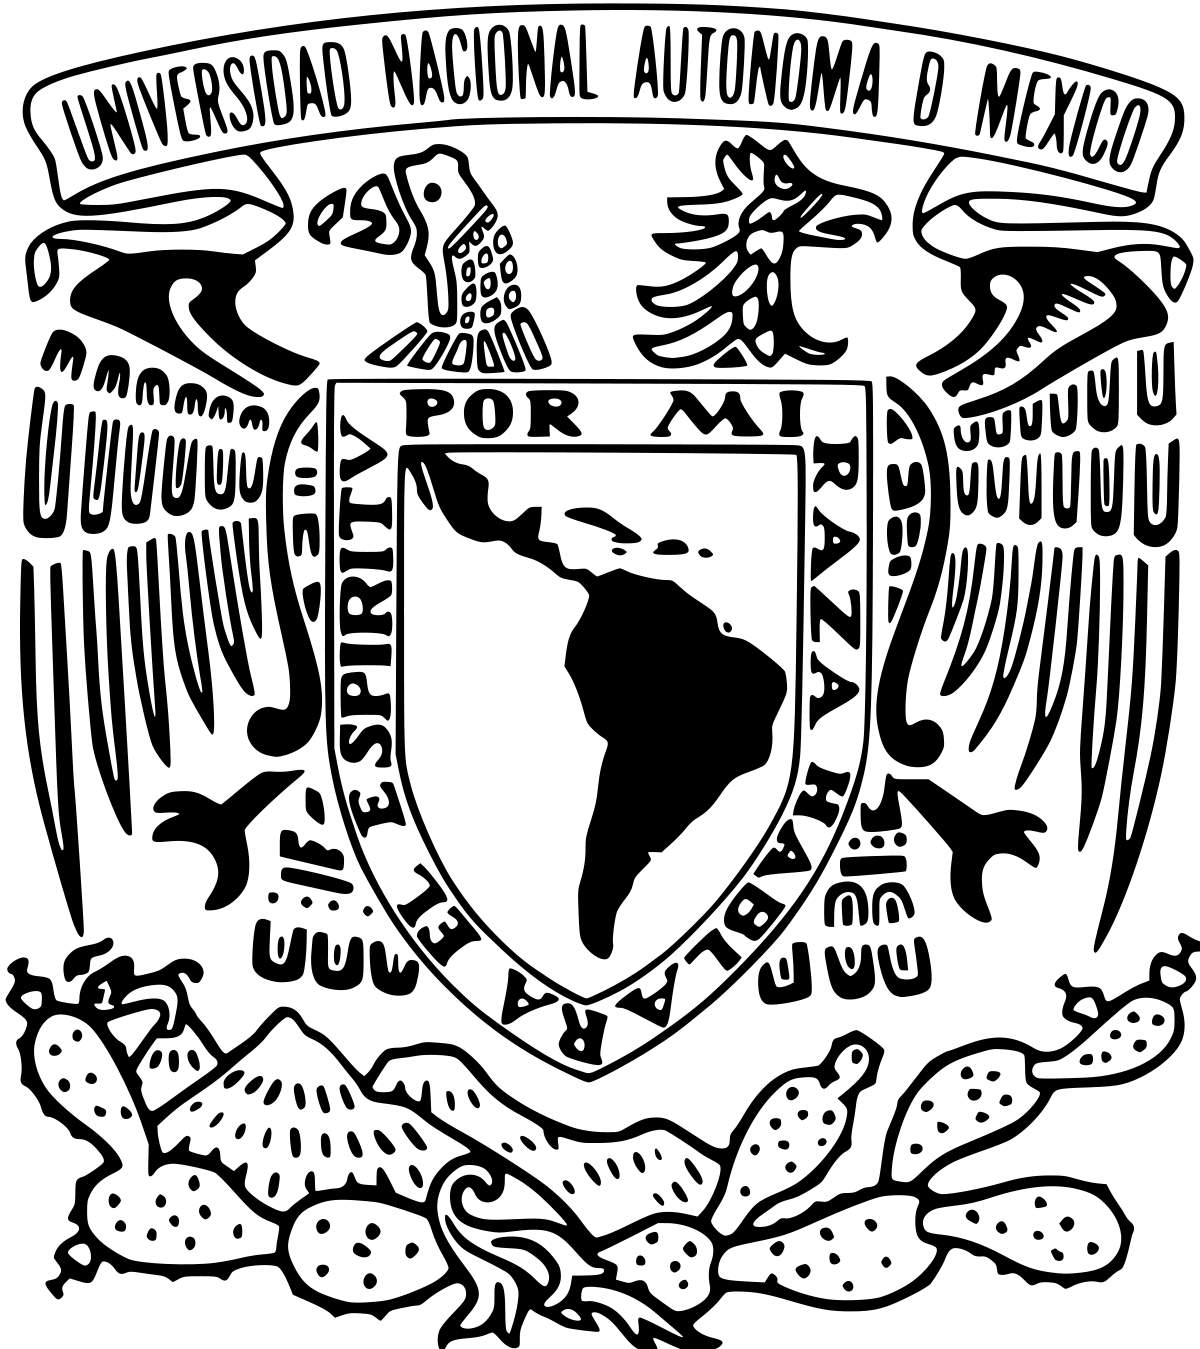
\includegraphics[width=3.5cm, height=3.5cm]{resources/Logo_UNAM.png}
		\end{center}
	\end{minipage}
	\begin{minipage}[c][0.195\textheight][t]{0.75\textwidth}
		\begin{center}
			\vspace{0.3cm}
			\textsc{\large Universidad Nacional Aut\'onoma de M\'exico}\\[0.5cm]
			\vspace{0.3cm}
			\hrule height2.5pt
			\vspace{.2cm}
			\hrule height1pt
			\vspace{.8cm}
			\textsc{Facultad de Ciencias}\\[0.5cm] %
		\end{center}
	\end{minipage}
	
	\begin{minipage}[c][0.81\textheight][t]{0.25\textwidth}
		\vspace*{5mm}
		\begin{center}
			\hskip2.0mm
			\vrule width1pt height13cm 
			\vspace{5mm}
			\hskip2pt
			\vrule width2.5pt height13cm
			\hskip2mm
			\vrule width1pt height13cm \\
			\vspace{5mm}
			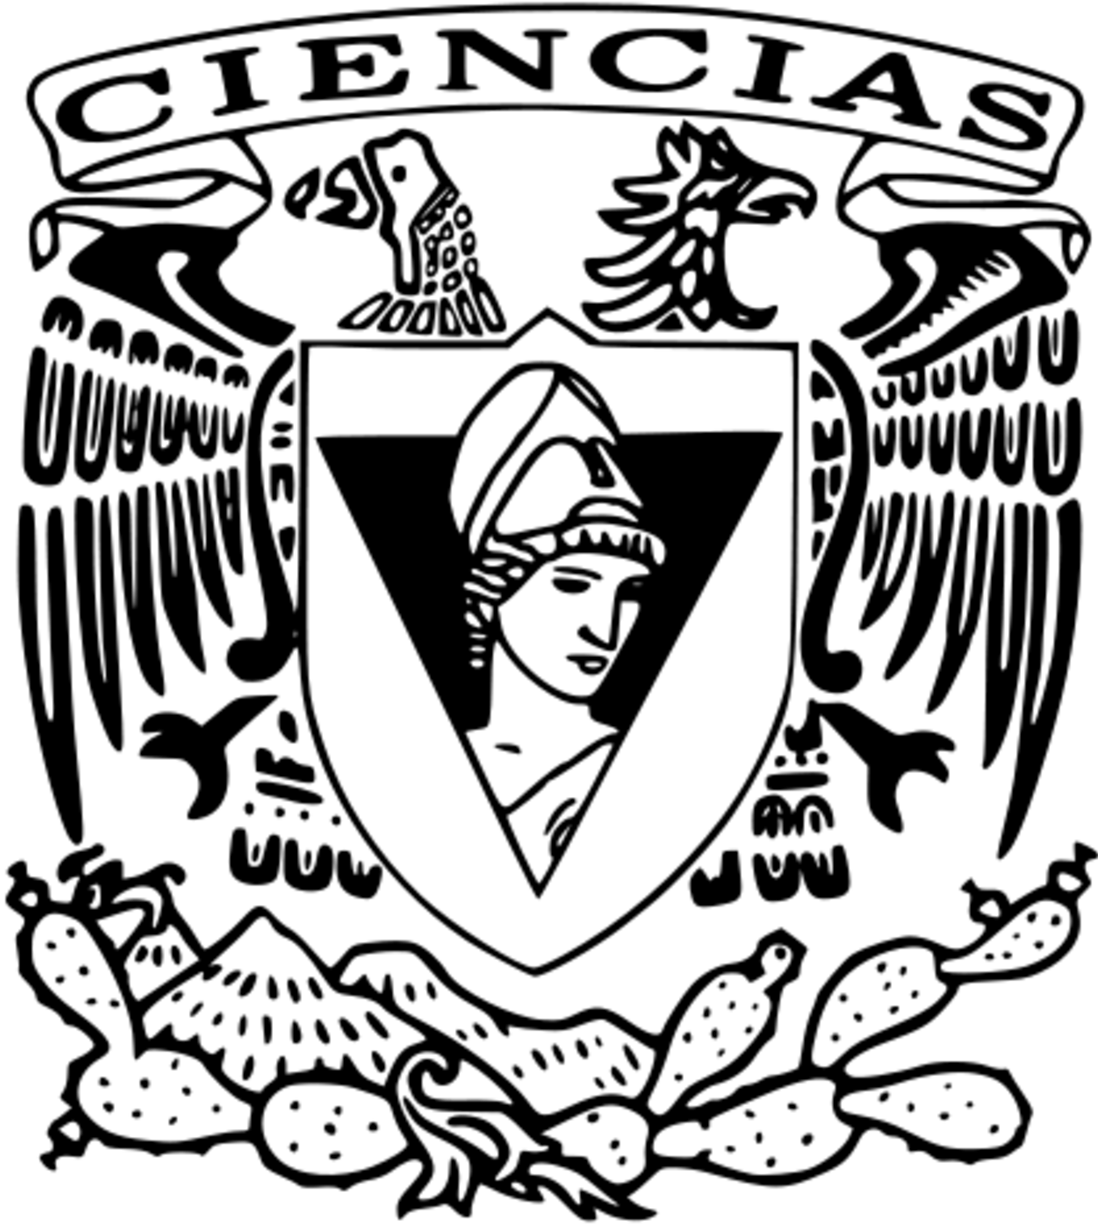
\includegraphics[height=4.0cm]{resources/Logo_FC.png}
		\end{center}
	\end{minipage}
	\begin{minipage}[c][0.81\textheight][t]{0.75\textwidth}
		\begin{center}
			\vspace{1cm}
			
			{\large\scshape Fundamentos de Bases de Datos - 7094}\\[.2in]
			
			\vspace{2cm}            
			
			\textsc{\LARGE \textbf{T}\hspace{1cm}\textbf{A}\hspace{1cm}\textbf{R}\hspace{1cm}\textbf{E}\hspace{1cm}\textbf{A}\hspace{1cm}\hspace{1cm}\textbf{4}}\\[2cm]
			\textsc{\Large{Equipo:}\normalsize \\
                \vspace{.3cm}
				\textbf{Del Monte Ortega Maryam Michelle - 320083527 \\
                \vspace{.2cm}
				\href{https://github.com/JuanSosaCiencias}{\textcolor{blue}{Sosa Romo Juan Mario - 320051926}} \\
                \vspace{.2cm}
				Castillo Hernández Antonio - 320017438 \\
                \vspace{.2cm}
                Erik Eduardo Gómez López - 320258211 \\
                \vspace{.2cm}
                Julio César Islas Espino - 320340594}}\\[0.5cm]     
			
			\textsc{{Fecha de entrega: \\ \textbf{10 de Octubre de 2024}}}\\[0.5cm]        
			
			\textsc{{Profesor: \\ \textbf{M. en I. Gerardo Avilés Rosas}}}\\[0.5cm]  
			
			\textsc{Ayudantes: \\ \textbf{Luis Enrique García Gómez \\ Kevin Jair Torres Valencia \\ Ricardo Badillo Macías \\ Rocío Aylin Huerta González
			} }
			
			
			\vspace{0.5cm}
		\end{center}
	\end{minipage}
\end{titlepage}

	
	\begin{center}
		\section*{\LARGE{Tarea 4}}
	\end{center}

    % Preguntas  
    \begin{center}
        \LARGE{\textbf{Preguntas}}\\
    \end{center}
    \normalsize
    
    \begin{enumerate}%[label=\alph*.]
        \item \begin{center}
    \textbf{Menciona 5 diferencias sentre almacenar la informacion utilizando un sistema de archivos o almacenarla utilizando una BDD.}
\end{center}

\begin{enumerate}
    \item \textbf{Estructura de Datos:} Los sistemas de archivos son simples colecciones de archivos sin relación entre ellos, mientras que             las bases de datos organizan los datos de manera estructurada y con relaciones lógicas.
    \item \textbf{Redundancia:} La redundancia de datos es alta en los sistemas de archivos, ya que los mismos datos pueden aparecer en                 múltiples lugares. En las bases de datos, la redundancia se minimiza mediante normalización.
    \item \textbf{Consistencia de Datos:} Los sistemas de archivos tienen problemas de inconsistencia cuando los datos se modifican en                 varios archivos. En las bases de datos, las actualizaciones se reflejan de manera consistente en todas las instancias de los datos.
    \item \textbf{Seguridad:} Los sistemas de archivos suelen ofrecer menos seguridad, mientras que las bases de datos incluyen medidas de             seguridad avanzadas como control de acceso y encriptación. 
    \item \textbf{Copia de Seguridad y recuperación:} Los sistemas de archivos no cuentan con mecanismos automatizados de respaldo y                     recuperación, mientras que las bases de datos generalmente incluyen estas funciones para proteger la información.\\
\end{enumerate}
\cite{guru99, sooluciona}

\vspace{.5cm}



        \item \textbf{¿Qué ventajas y desventajas encuentras al trabajar con un Sistema de Bases de Datos
considerando que se planea implantar este sistema en una empresa de telemarketing?} \\

En primera instancia tenemos que reconocer que el telemarketing es una técnica publicitaria que es utilizada por las empresas para contactar con potenciales clientes y hablarles acerca de sus productos o servicios . \\

Hay muchas empresas a lo largo del mundo que hacen de esta estrategia su principal manera de operar, catalogándose en mayor o menor medida como empresas de telemarketing y si bien cada empresa decide como gestionar sus recursos para así poder llegar a su publico objetivo, el telemarketing cuenta con una serie de ventajas y desventajas enumeradas de la siguiente manera las cuales pueden hacer que una empresa se decante por este sistema o no: \\


\begin{table}[h!]
    \centering
    \begin{tabular}{|p{6cm}||p{6cm}|}
        \hline
        \textcolor{blue}{\textbf{Ventajas}} & \textcolor{Red}{\textbf{Desventajas}} \\ \hline 
        Se tiene un trato mas directo con los potenciales clientes & Si se utiliza de manera inadecuada puede afectar negativamente a la reputación de la empresa \\ \hline
        Permite entrar en contacto con un gran número de clientes en poco tiempo & En algunos países existen ciertas restricciones para esta clase de técnicas \\ \hline 
        Permite ofrecer una gran cantidad de información sobre el producto o servicio en cuestión  & Requiere una inversión en formar a los agentes y que estos sigan las buenas practicas de la empresa \\ \hline
        Se puede llamar a cualquier parte del mundo, lo cual asegura que nuestra empresa pueda darse a conocer en otras fronteras & La tasa de conversión es baja\\ \hline
    \end{tabular}
    \caption{Ventajas y desventajas de un Sistema de Telemarketing \cite{boada_cyberclick_2023}} 
\end{table}

Así mismo el telemarketing puede utilizarse de distintas maneras y estas varían de acuerdo a la campaña y objetivos de la empresa. Pero volviendo al punto principal de la pregunta, algunas de las posibles ventajas y desventajas de implemmentar un sistema de base de datos en alguna empresa de telemarketing podrian ser las siguientes:\\


\begin{table}[h!]
    \centering
    \begin{tabular}{|p{6cm}||p{6cm}|}
        \hline
        \textcolor{green}{\textbf{Ventajas}} & \textcolor{purple}{\textbf{Desventajas}} \\ \hline
        Organización y gestión eficiente de datos & Altos costos de implementación y mantenimiento continuo. \\ \hline
        Generación de análisis detallados e historial de datos. & Trabajo extra para integración con sistemas existentes y necesidad de capacitación del personal. \\ \hline
         Automatiza las tareas repetitivas y hay una reducción de errores manuales. & Riesgo de interrupciones por fallos del sistema y necesidad de ajustes por actualizaciones. \\ \hline
        Tiene la capacidad para manejar más datos y mas personalización según necesidades específicas. &  Riesgos de seguridad y necesidad de cumplir con normativas de privacidad. \\ \hline
        Existe un control de acceso a datos sensibles y así como también un respaldo de datos. & Existen riesgos por parte de entradas de datos incorrectos y problemas de duplicados. \\ \hline
    \end{tabular}
    \caption{Ventajas y desventajas de un Sistema de BD en una empresa de telemarketing}
    \cite{adSalsa_2024}
\end{table}
   
        \begin{enumerate}[label=\alph*.]
            \item \textbf{Obtener toda la información de los clientes que viven en Seatle o en San Francisco, que pertenezcan al segmento
corporate que hayan solicitado una orden en el segundo trimestre de 2014. Mostrar la información ordenada por la
cantidad solicitada.} \vspace{.3cm}

La verdad es que la sintaxis de la pregunta deja poco claro lo que se necesita pero yo lo interprete de la siguiente manera:

\begin{center}
    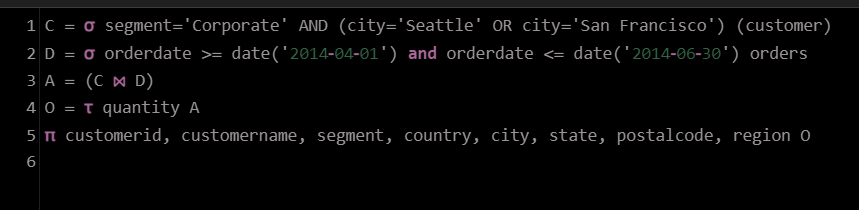
\includegraphics[width=14cm]{resources/pregunta2/2.1.1.png}
\end{center}

La idea es la siguiente, comenzamos por seleccionar a los clientes que viven en Seatle o en San Francisco, que pertenezcan al segmento corporate, eso es una mini consulta. Luego seleccionamos las ordenes que se hicieron en el segundo trimestre de 2014, eso es otra mini consulta. Luego unimos ambas consultas, finalmente ordenamos por la cantidad solicitada, aqui es donde no estoy seguro de si ahi acaba nuestra consulta o, como dice que solo quiere la información de los clientes tenemos que solo regresarle las columnas relevantes (si no hacemos el siguiente paso se van a repetir clientes porque tienen varios pedidos, igual otra opcion es agrupar por cliente), entonces decidi incluir esta ultima aunque si no es necesario podriamos parar ahi, entonces solo proyectamos sobre las columnas de costumer sobre la consulta anterior.

Esto nos regresa la siguiente tabla:

\begin{center}
    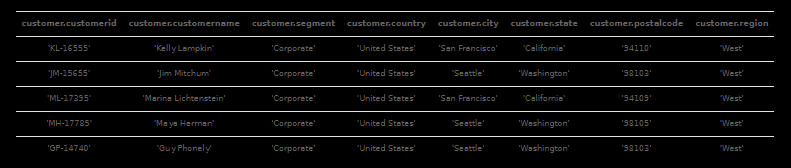
\includegraphics[width=14cm]{resources/pregunta2/2.1.2.png}
\end{center}

Como se ve esto regresa toda la información de los clientes en la forma que se solicita con el detalle de no incluir detalle de la orden.

\newpage 
            \item \textbf{Obtener una relación de los productos que pertenecen a la categoría Office Supplies con precio mayor de $300 y menor de $600, pero que no hayan sido solicitados en ninguna orden.} \vspace{.3cm}

\begin{center}
    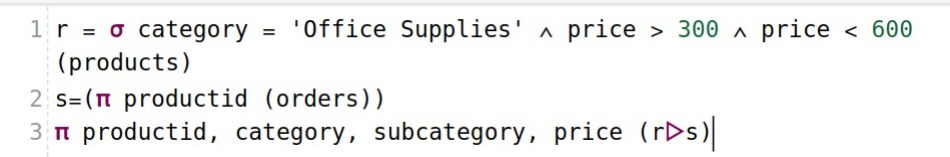
\includegraphics[width=5cm]{resources/pregunta2/2.2.1.jpg}
\end{center}

Esta consulta resulta de la abstracción de algunos conceptos:
\begin{itemize}
    \item \textbf{r} tabla de products con las condiciones solicitadas de precio mayor de $300 y menor de $600
    \item  \textbf{s} es la tabla de los ids de productos que han sido solicitados en alguna orden
    \item  \textbf{$r \vartriangleright q$} es la tabla de productos de la categoría Office Supplies con precio mayor de $300 y menor de $600 y que no coiciden o no estan dentro de la tabla de ids de productos solicitados en alguna orden.
\end{itemize}

El resultado es:

\begin{center}
    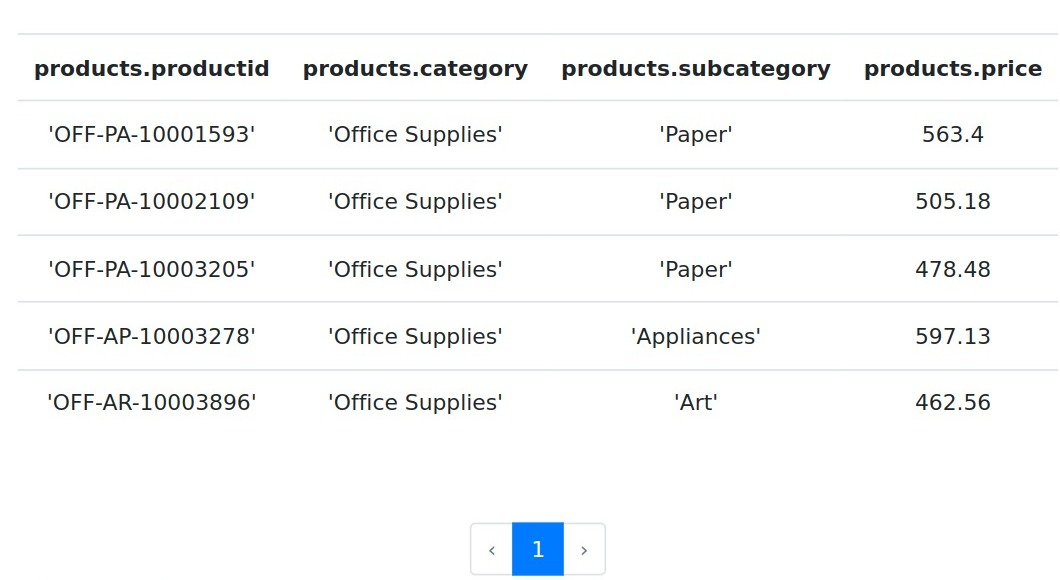
\includegraphics[width=5cm]{resources/pregunta2/2.2.2}
\end{center}


            \item \textbf{Obtener el nombre de todos los clientes que vivan en la región West y hayan solicitados productos de las categorías Technology o Furniture. El pedido debió de solicitarse en 2106 y el modo de envío debe ser Standard Class.}

Asumiré que cuando dice "El pedido debió de solicitarse en 2106" se refiere al 2016. 

\begin{center}
    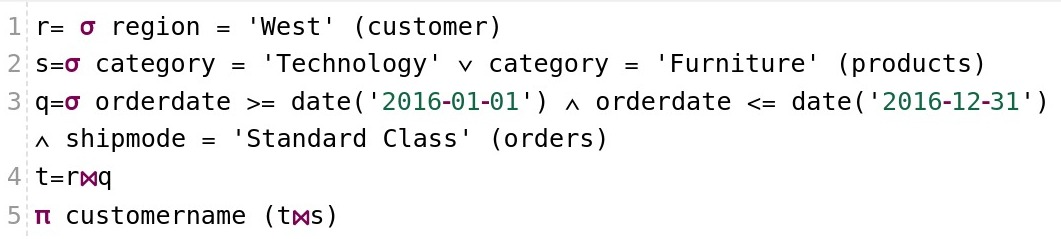
\includegraphics[width=5cm]{resources/pregunta2/2.3.1}
\end{center}
Para esta consulta 
\begin{itemize}
    \item \textbf{r} es la tabla de clientes de la región West
    \item \textbf{s} es la tabla de productos de categoría Technology o Furniture
    \item \textbf{q} es la tabla de pedidos enviados en modo Standard Class en el 2016
    \item \textbf{t} es la relacion de clientes que viven en West que hicieron un pedido en modo Standard Class en el 2016
    \item \textbf{t \join s} es la relacion de clientes que viven en West que hicieron un pedido en modo Standard Class en el 2016, y ademas su producto es de categoria Technology o Furniture
\end{itemize}

El resultado es:
\begin{center}
    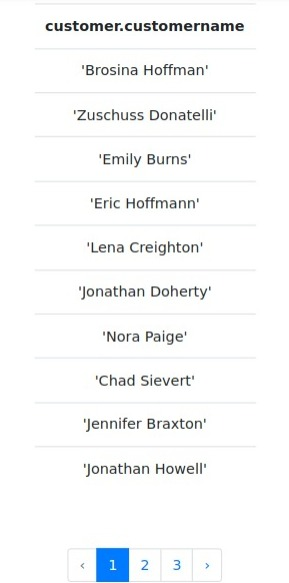
\includegraphics[width=5cm]{resources/pregunta2/2.3.2}
\end{center}

Nótese que primero hacemos join de r con q, ya que el atributo en común es customerid, de otra forma obtendríamos el producto cartesiano, lo cuál es demasiado costoso en términos de recursos. 
\begin{center}
    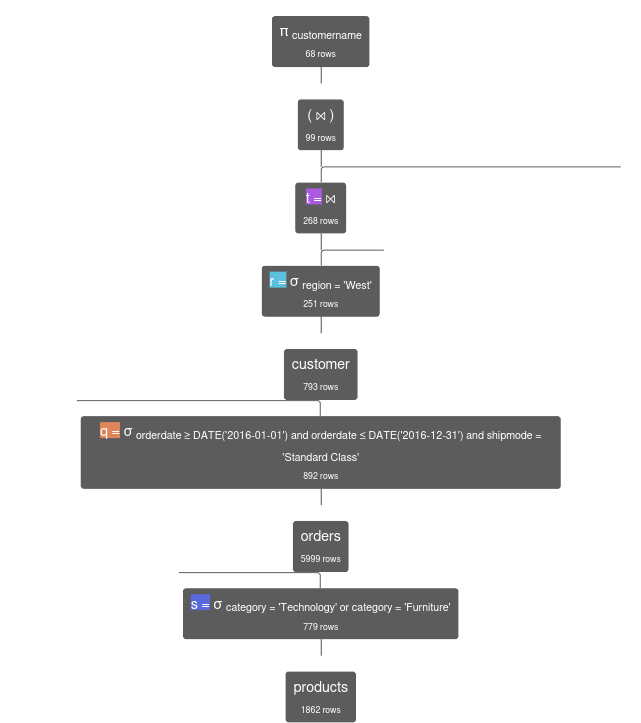
\includegraphics[width=5cm]{resources/pregunta2/2.3.3}
\end{center}

            \item Toda la información de los clientes del segmento \textbf{Corporate} que realizaron una orden con modo de envío \textbf{First Class}
y que no viven en \textbf{California}.
            \item Obtener el \textbf{estado, segmento} y el \textbf{total de clientes} que no han solicitado \textbf{ninguna orden}. \\

Dado esto, \textit{seleccionamos} todos los clientes de la relación \textit{customer}, almacenando dichas tuplas en una relación temporal \textit{clientes}. Luego, seleccionamos los IDs de los clientes que han realizado órdenes de la relación \textit{orders}, almacenando dichas tuplas en una relación temporal \textit{clientes\_con\_ordenes}. A continuación, obtenemos los IDs de los clientes que no han realizado ninguna orden mediante la operación de diferencia de conjuntos entre \textit{clientes} y \textit{clientes\_con\_ordenes}, almacenando el resultado en relación temporal \textit{clientes\_sin\_ordenes}. Finalmente, utilizamos el operador de proyección para obtener el \textbf{estado, segmento} y el \textbf{total de clientes} que no han solicitado \textbf{ninguna orden}. \\

La consulta en álgebra relacional se vería mas o menos de la siguiente manera: \\

\begin{center}
    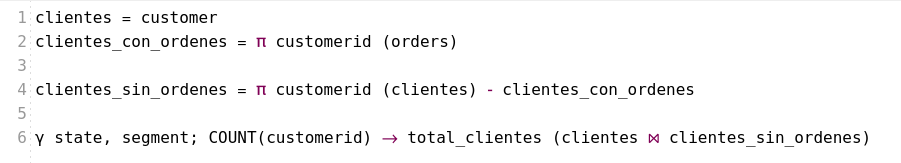
\includegraphics[width=14cm]{resources/pregunta2/2.5.1.png} \\
\end{center}

El árbol de la consulta: \\

\begin{center}
    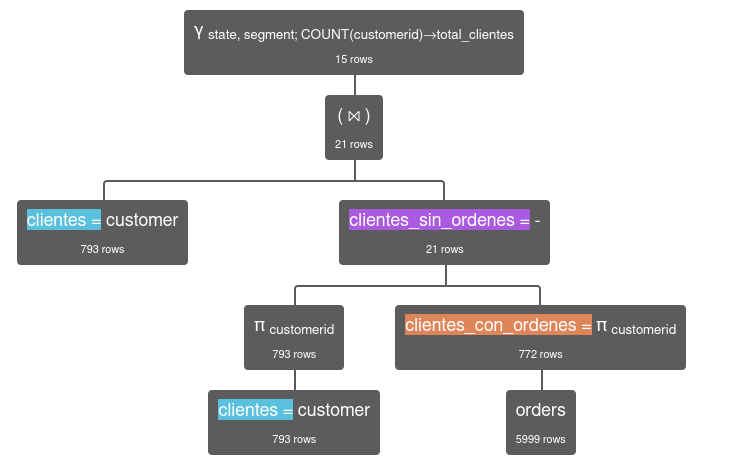
\includegraphics[width=14cm]{resources/pregunta2/2.5.2.png} \\
\end{center}

y la tabla resultante: \\

\begin{center}
    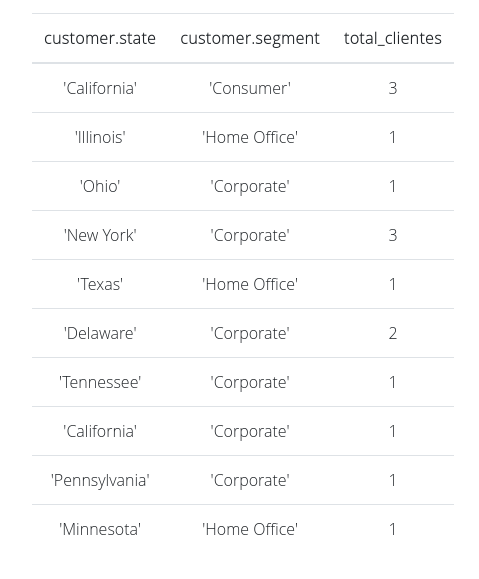
\includegraphics[width=10cm]{resources/pregunta2/2.5.3.png} \\
\end{center}

            \item \textbf{Una lista que muestre la región, el estado y el total de clientes que se tienen, considerando que los clientes deben
haber realizado órdenes con al menos 6 productos durante 2014 o 2015. Ordenar la información por región y estado..} \vspace{.3cm}

Primero el Álgebra Relacional es:

\begin{center}
    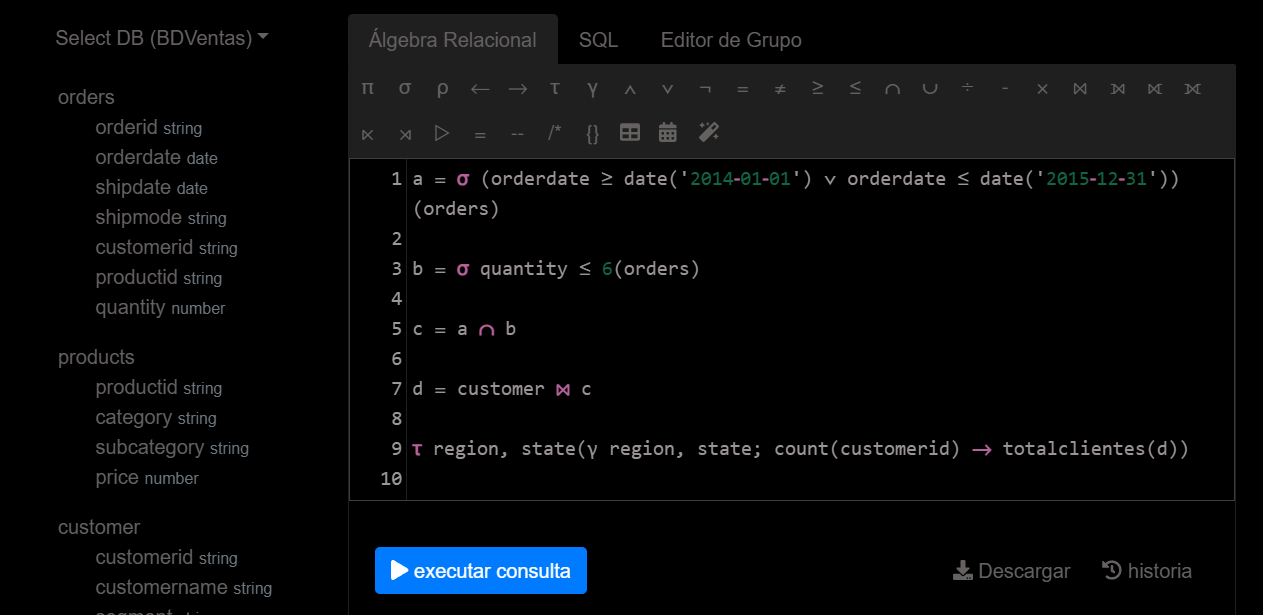
\includegraphics[width=14cm]{resources/pregunta2/2.6.1.png}
\end{center}


El resultado de las tablas es:

\begin{center}
    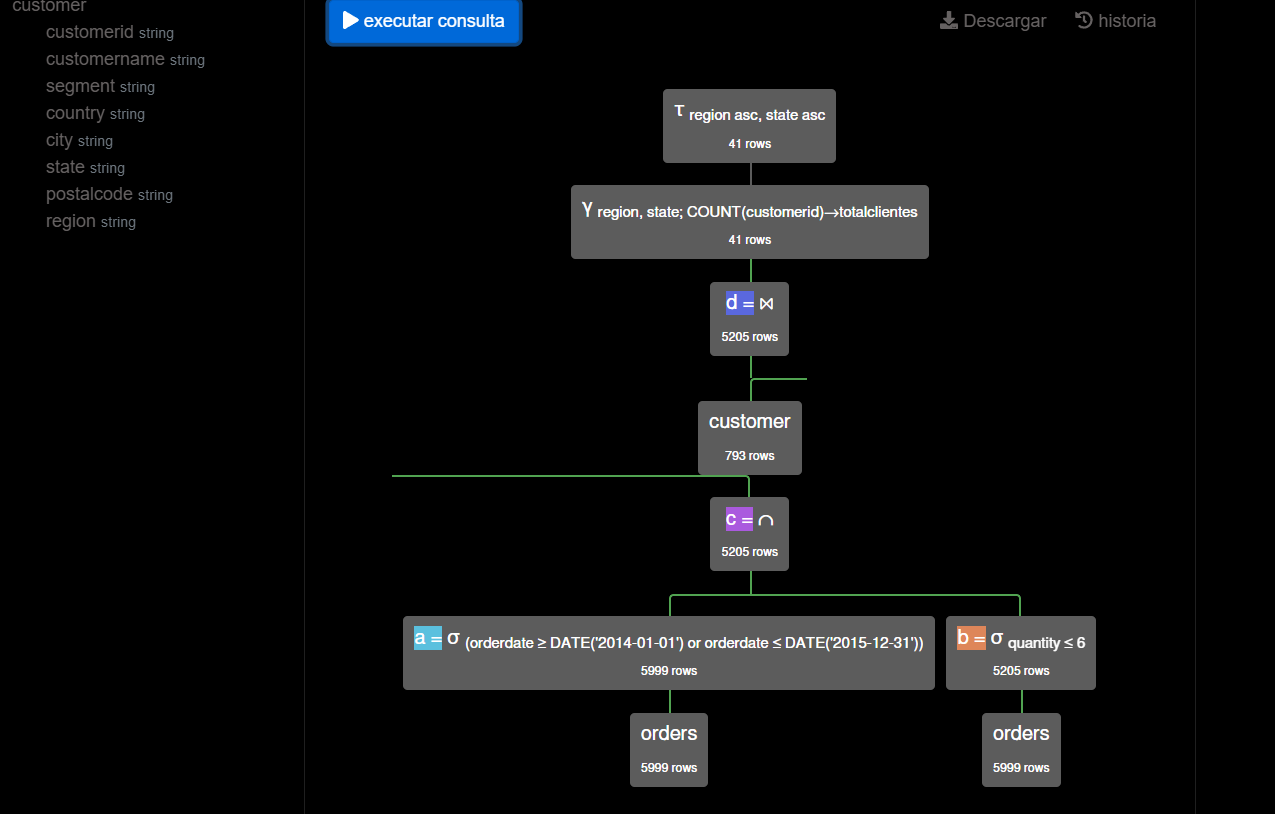
\includegraphics[width=14cm]{resources/pregunta2/2.6.2.png}
\end{center}


\begin{center}
    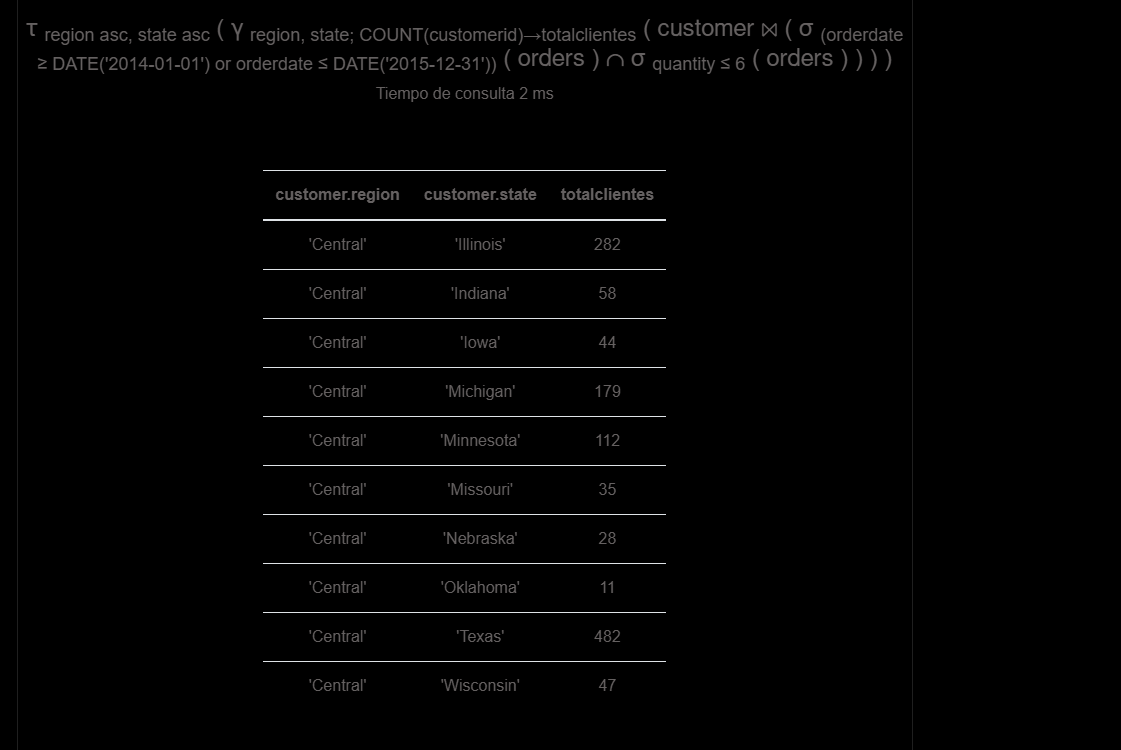
\includegraphics[width=14cm]{resources/pregunta2/2.6.3.png}
\end{center}

            \item \textbf{Obtener el modo de envío y categoría que más productos ha vendido.}

El enunciado es bastante ambiguo. No hay muchos detalles así que realizamos lo siguiente:

Obtendremos las categorías y modos de envio que mas productos han vendido combinaciones diferentes

\begin{center}
    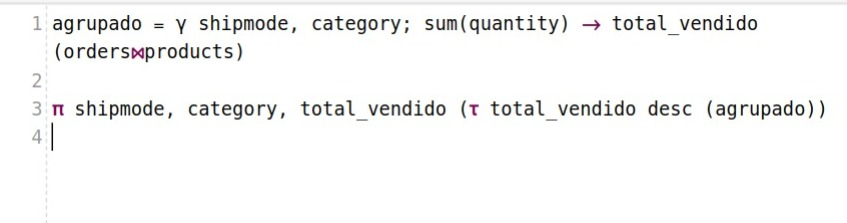
\includegraphics[width=14cm]{resources/pregunta2/2.7.1} \\
\end{center}
El resultado:
\begin{center}
    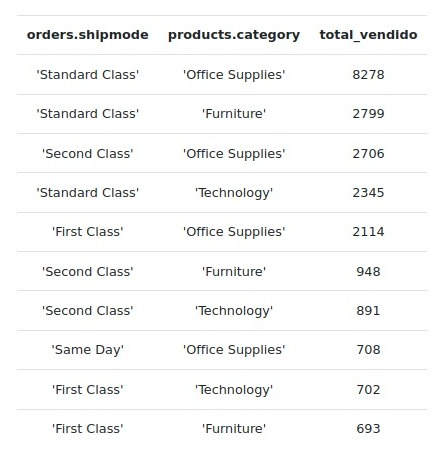
\includegraphics[width=14cm]{resources/pregunta2/2.7.2} \\
\end{center}

            \item Una tabla con la venta promedio, venta total, mayor venta, menor venta, y total de órdenes, por región, estado y
ciudad. La venta promedio debe estar entre $ \$900$ y $\$1,500.$

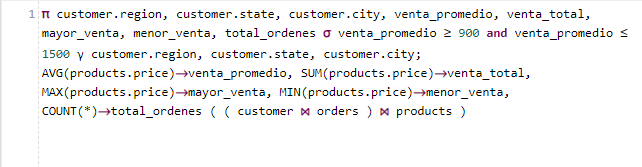
\includegraphics[width= 15cm]{resources/2h-1.png}
\vspace{0.15cm}
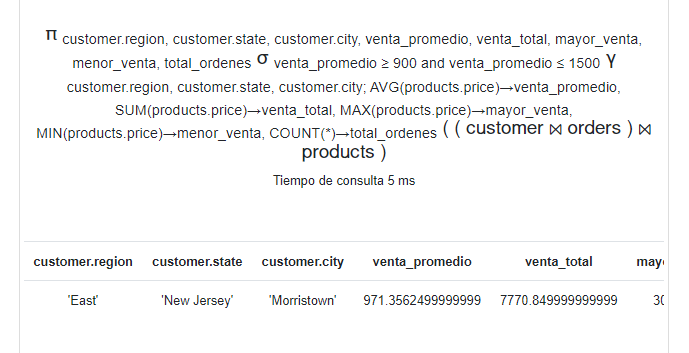
\includegraphics[width= 15cm]{resources/2h-2.png}
\vspace{0.15cm}
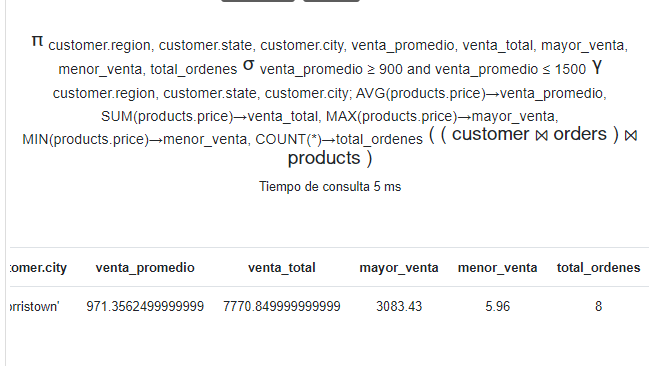
\includegraphics[width= 15cm]{resources/2h-3.png}
            \item El estado que ha realizado la mayor cantidad de órdenes. Se debe mostrar también el total de ordenes que haya
entregado.

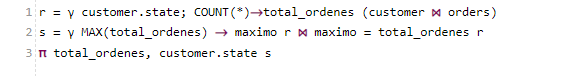
\includegraphics[width= 15cm]{resources/2i-1.png}
\vspace{0.15cm}
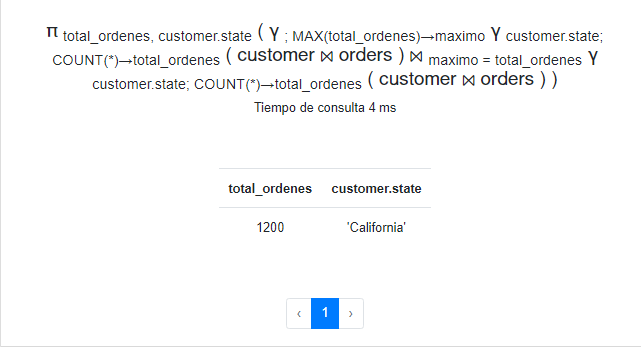
\includegraphics[width= 15cm]{resources/2i-2.png}
            \item La información del cliente que menos órdenes haya efectuado. Mostrar el número de órdenes que ha realizado.

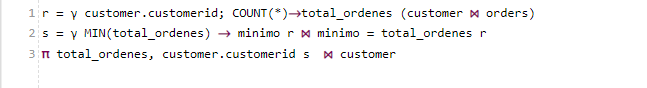
\includegraphics[width= 15cm]{resources/2j-1.png}
\vspace{0.15cm}
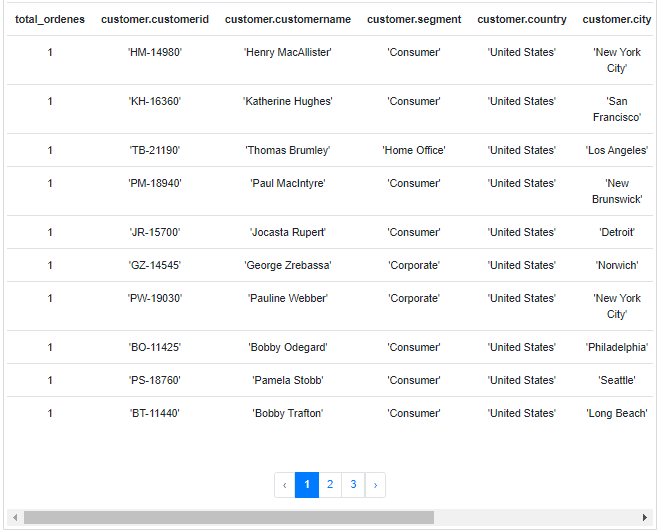
\includegraphics[width= 15cm]{resources/2j-2.png}
        \end{enumerate}
        \item \textbf{Investiga que cuáles son las Reglas de Codd y explica con tus propias palabras cada una de ellas. Indica por qué
consideras que son importantes.}\vspace{.3cm}

        \begin{enumerate}[label=\alph*.]
            \item \textbf{Borrar toda la información del cliente Paul Stevenson.}

Para esta consulta en algebra relacional solo deberémos descartar cualquier fila que coincida con Paul Stevenson

\begin{center}
    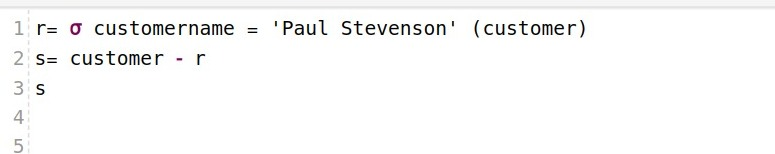
\includegraphics[width=5cm]{resources/pregunta2/3.1.1}
\end{center}

Así obtenemos el siguiente árbol de consulta
\begin{center}
    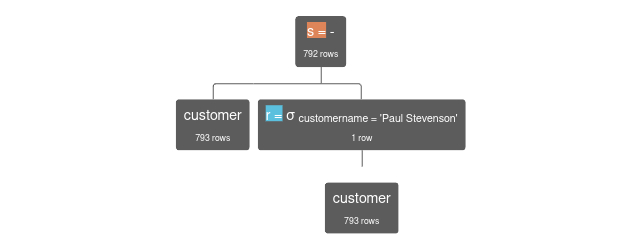
\includegraphics[width=7cm]{resources/pregunta2/3.1.2}
\end{center}
Y el resultado:
\begin{center}
    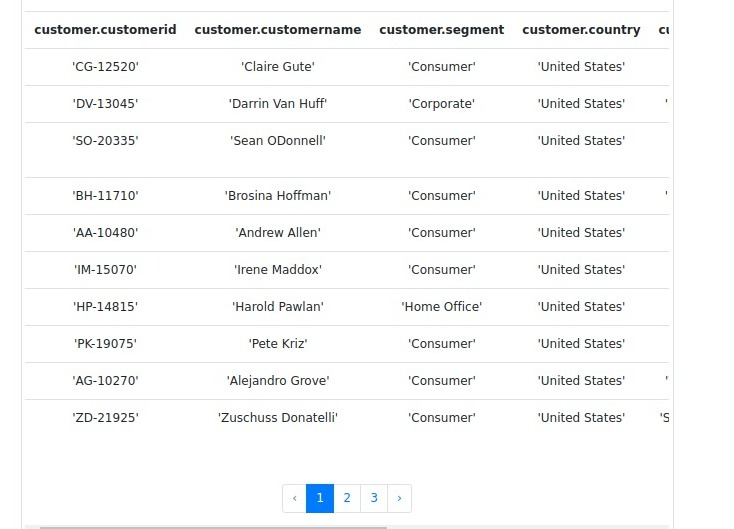
\includegraphics[width=9cm]{resources/pregunta2/3.1.3}
\end{center}

Si lo hacemos con sql obtenemos los mismos resultados
\begin{center}
    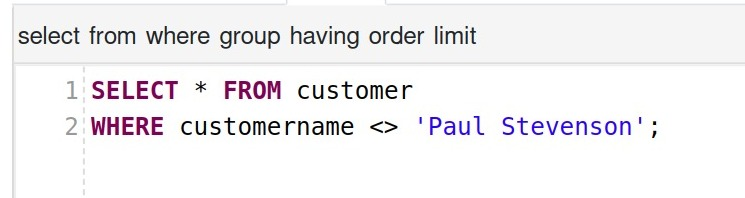
\includegraphics[width=5cm]{resources/pregunta2/3.1.4}
\end{center}
 
            \item Borrar todas las órdenes de la ciudad Utah que tengan artículos de la subcategoría \textbf{Tables}. \\

En este caso, lo primero que hacemos es realizar un natural join entre \textit{orders}, \textit{customer} y \textit{products}, almacenando dicho join en una relación temporal \textit{r}. Luego, seleccionamos las tuplas que sean de la ciudad \textbf{Utah} y que tengan artículos de la subcategoría \textbf{Tables}, guardando estas tuplas en otra relación temporal \textit{s}. A continuación, hacemos una proyección de los IDs de la relación \textit{s} creada anteriormente (llamamos a esto \textit{ordenes\_a\_borrar}). Finalmente, hacemos una diferencia entre \textit{orders} y el join natural derivado de \textit{orders} y \textit{ordenes\_a\_borrar}. \\

La consulta en algebra relacional se veria de la siguiente manera: \\

\begin{center}
    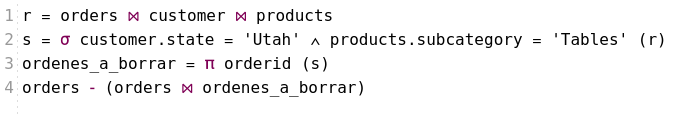
\includegraphics[width=14cm]{resources/pregunta2/3.2.1.png} \\
\end{center}

Ahora el árbol de la consulta: \\

\begin{center}
    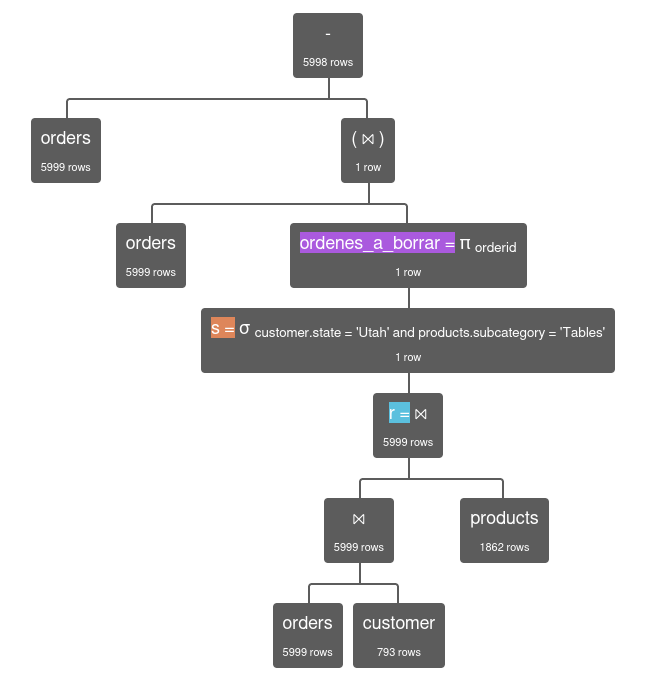
\includegraphics[width=10cm]{resources/pregunta2/3.2.2.png} \\
\end{center}

y forma de la tabla resultante: \\
\begin{center}
    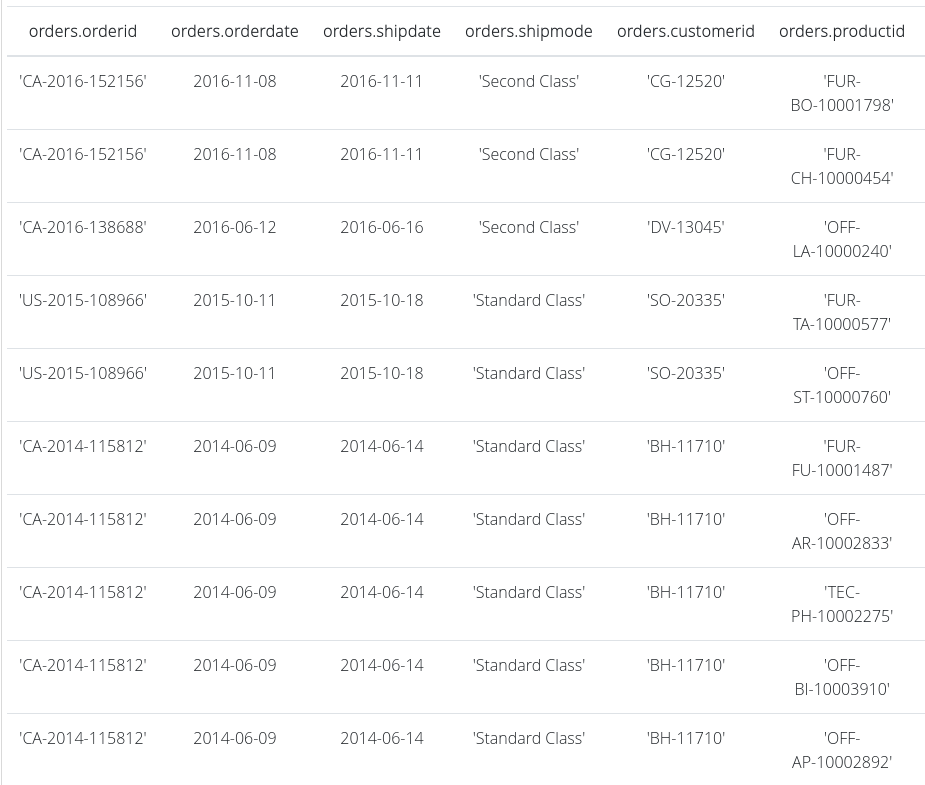
\includegraphics[width=14cm]{resources/pregunta2/3.2.3.png} \\
\end{center}
            \item \textbf{La clienta Lena Cacioppo compró un producto de cada subcategoría de Furniture. Deberás elegir los productos que
desees e indicar como parte de esta consulta, la información que se agregará en cada caso.} \vspace{.3cm}

Primero el Álgebra Relacional es:

\begin{center}
    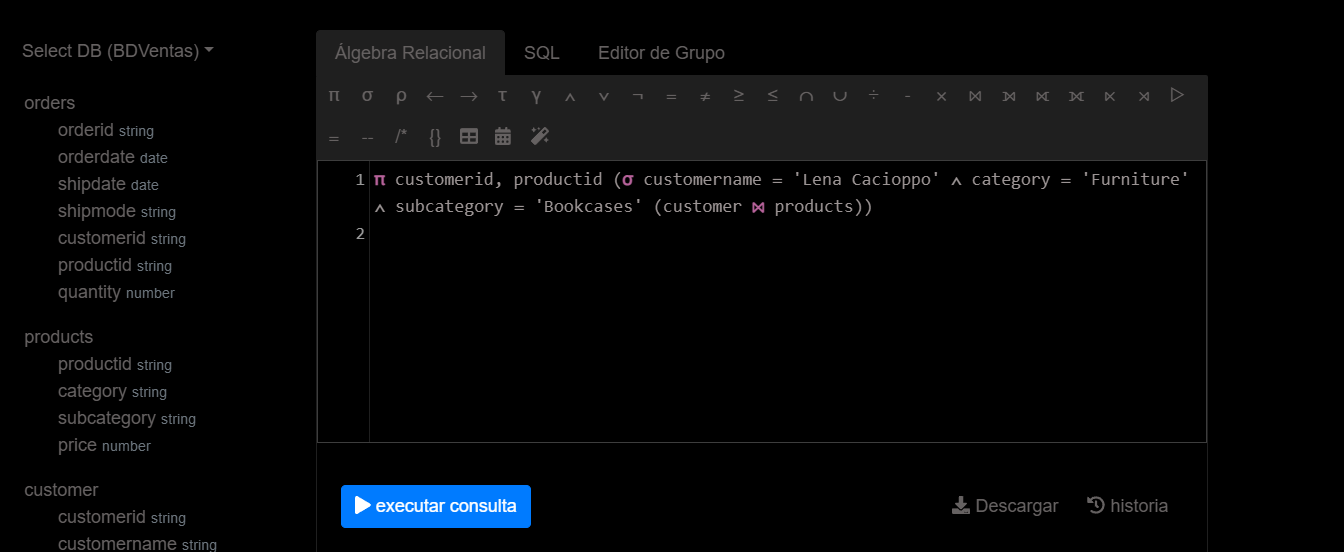
\includegraphics[width=14cm]{resources/pregunta2/3.3.1.png}
\end{center}


El resultado de las tablas es:

\begin{center}
    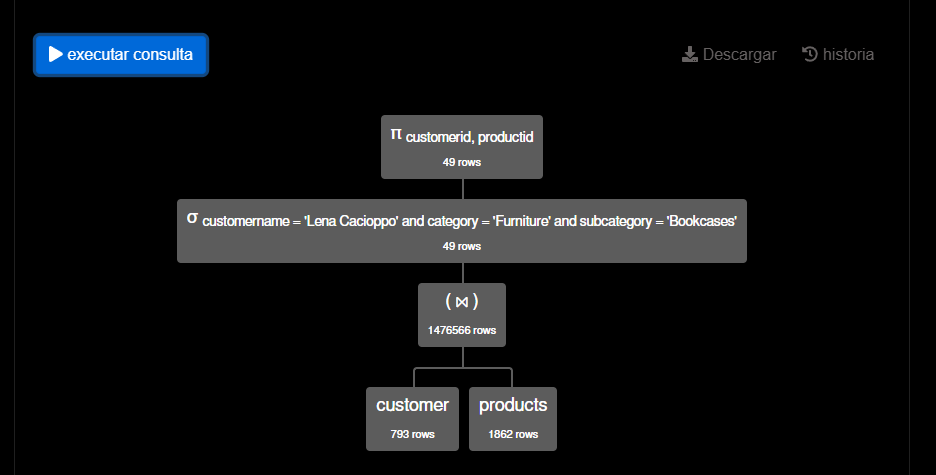
\includegraphics[width=14cm]{resources/pregunta2/3.3.3.png}
\end{center}

\begin{center}
    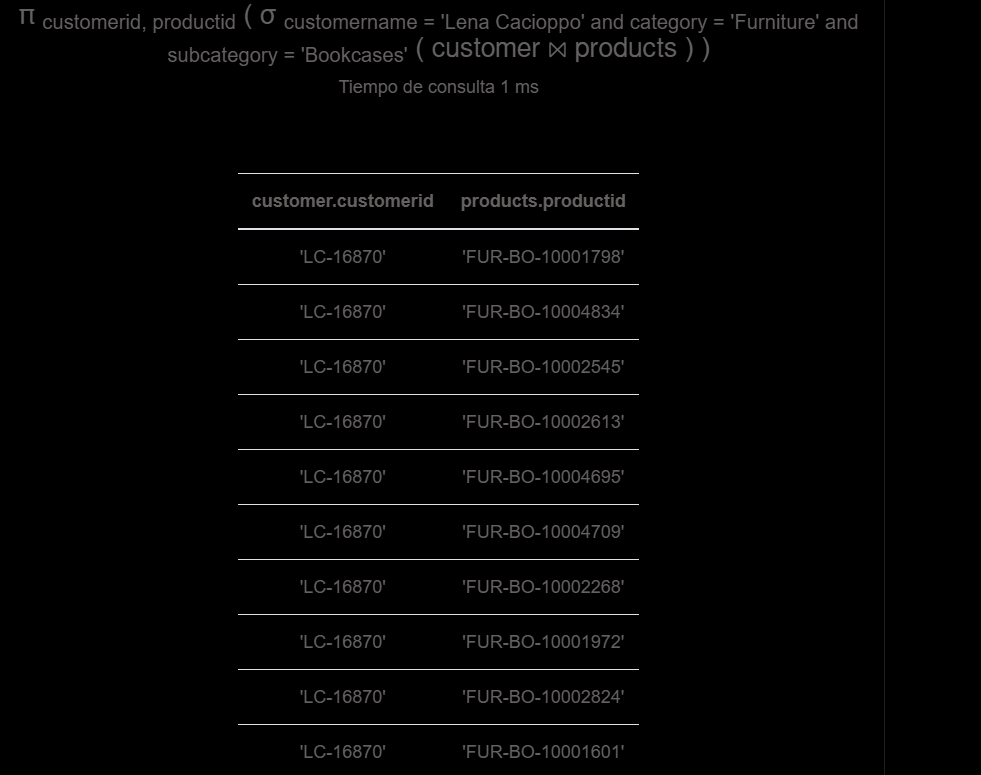
\includegraphics[width=14cm]{resources/pregunta2/3.3.2.png}
\end{center}

            \item Aumentar los precios de productos de la subcategoría Phones en un $8\%$.

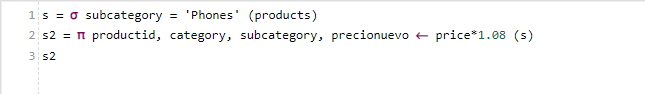
\includegraphics[width= 15cm]{resources/3d-1.png}

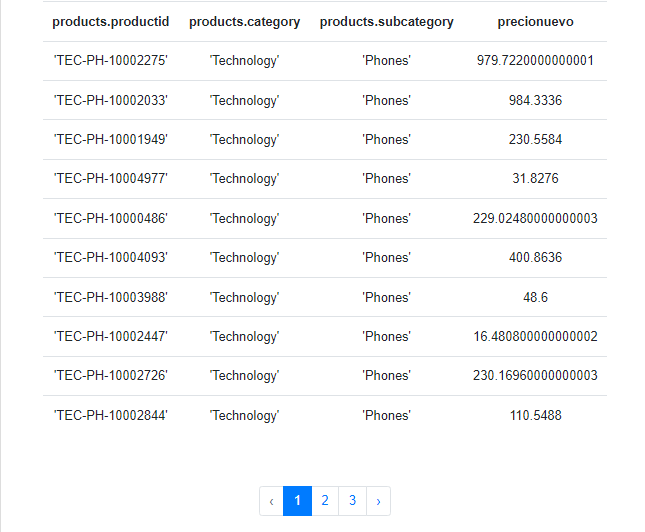
\includegraphics[width= 15cm]{resources/3d-2.png}
            \item \textbf{Disminuir 8\% los precios de los productos de la categoría Furniture cuyo precio sea de \$600 a \$900. Aumentar en
un 5\% los precios de los productos de la categoría Technology y subcategoría Machines.} \vspace{.3cm}

Para esta consulta  use el video '07 Álgebra Relacional | Actualización | Operaciones de mantenimiento de datos', al final use esta consulta:

\begin{center}
    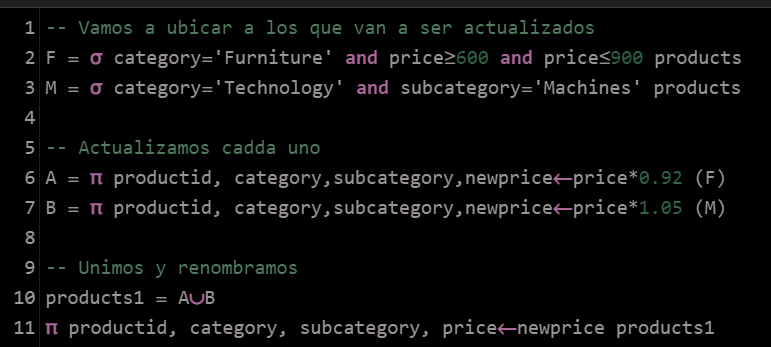
\includegraphics[width=14cm]{resources/pregunta2/3.5.1.png}
\end{center}

De manera que me quedo la siguiente Actualización:

\begin{center}
    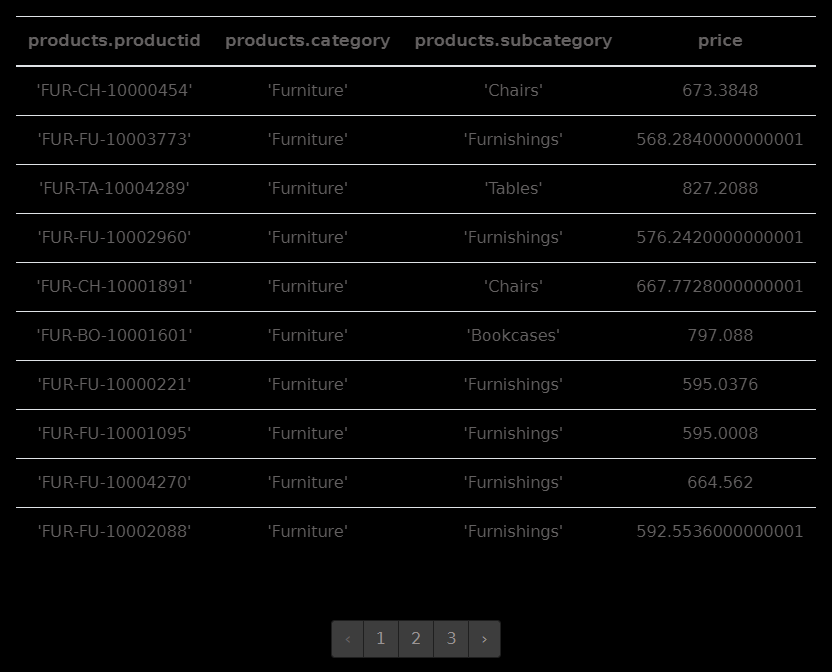
\includegraphics[width=14cm]{resources/pregunta2/3.5.2.png}
\end{center}

Ojo que esta solo contiene la tabla de los productos con los precios actualizados como se ve en el video, no contiene toda la lista de productos pero seria tan facil como eliminar las tuplas que se estan seleccionando, e insertar estas nuevas, no lo hice pues no lo hizo el profe :v.
\newpage        
        \end{enumerate}
    \end{enumerate}
    \newpage
    
% \printbibliography
  
\end{document}